\documentclass{beamer}
\beamertemplatenavigationsymbolsempty

\usecolortheme{beaver}
\setbeamertemplate{blocks}[rounded=true, shadow=true]
\setbeamertemplate{footline}[page number]
\setbeamercolor{itemize item}{fg=red}
\setbeamercolor{enumerate item}{fg=red}

\usepackage[utf8]{inputenc}
\usepackage[english,russian]{babel}
\usepackage{amssymb,amsfonts,amsmath,mathtext, dsfont}
\usepackage{makecell} % diaghead in a table
\usepackage{subfig}
\usepackage{tabularx}
\usepackage{array}
\usepackage{multicol, multirow}
\usepackage{hyperref}
\usepackage{hhline}

\usepackage{tikz}
\usetikzlibrary{matrix}

\newcommand{\bx}{\mathbf{x}}
\newcommand{\by}{\mathbf{y}}
\newcommand{\bz}{\mathbf{z}}
\newcommand{\bw}{\mathbf{w}}
\newcommand{\bY}{\mathbf{Y}}
\newcommand{\bX}{\mathbf{X}}
\newcommand{\dH}{\mathds{H}}

\newcommand{\T}{^{\mathsf{T}}}

\addto\captionsrussian{\renewcommand{\figurename}{}}

\graphicspath{{../figures/}}

\title[\hbox to 56mm{Определение фазы}]{Восстановление траектории \\ движения руки по видео}
\author[Э.\,А. Владимиров]{Владимиров Эдуард Анатольевич}
\institute{Московский физико-технический институт}
\date{\footnotesize
	\par\smallskip\emph{Курс:} Моя первая научная статья
	\par\smallskip\emph{Эксперт:} Р.\,В.~Исаченко
	\par\smallskip\emph{Консультанты:} А.\,Д.~Курдюкова
	\par\bigskip\small 2022}

\def\vec#1{\mathchoice{\mbox{\boldmath$\displaystyle#1$}}
	{\mbox{\boldmath$\textstyle#1$}} {\mbox{\boldmath$\scriptstyle#1$}} {\mbox{\boldmath$\scriptscriptstyle#1$}}}

\begin{document}
	\begin{frame}
		\thispagestyle{empty}
		\maketitle
	\end{frame}

	\begin{frame}{Восстановление траектории}
		
		\begin{alertblock}{Задача}
			Объединение методов канонического корреляционного анализа и метода Сугихары.
		\end{alertblock}
		
		\begin{alertblock}{Проблема}
			Построение скрытого пространства по временному ряду и выбор функции согласования латентных проекций
		\end{alertblock}
		
		\begin{alertblock}{Решение}
			Обучение автоэнкодеров и использование меры наличия причинно-следственной связи в функции согласования.
		\end{alertblock}
	\end{frame}

	\begin{frame}[fragile]{Методы понижения размерности и метод Сугихары}
		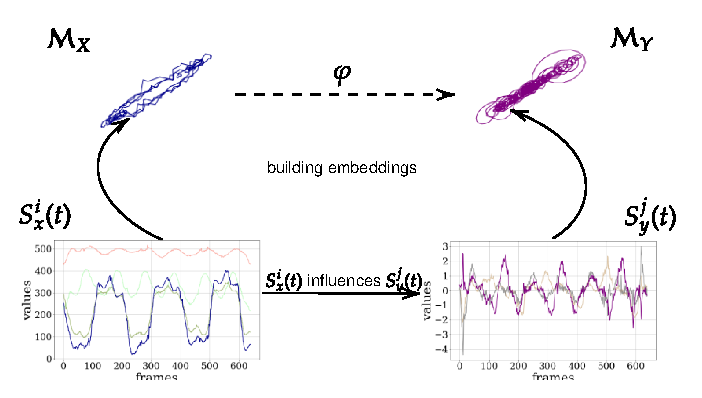
\includegraphics[height=5cm]{block_scheme_4.pdf}
				
		\begin{multicols}{2}
		\begin{tikzpicture}[scale=0.22]
			\matrix (m) [matrix of math nodes,row sep=3em,column sep=4em,minimum width=2em]
			{
				\underset{n \times d}{\bX} & \underset{n \times s}{\bY} \\
				\underset{n \times K}{\mathbf{T}} & \underset{n \times K}{\mathbf{U}} \\};
			\path[-stealth]
			(m-2-1) edge node [right] {$P^T$} (m-1-1)
			(m-2-2) edge node [left] {$Q^T$} (m-1-2)
			(m-1-1) edge [bend right] node [left] {$A$} (m-2-1)
			(m-1-2) edge [bend left] node [right] {$B$} (m-2-2)
			(m-2-1) edge [<->] node [above] {$cov$} (m-2-2)
			(m-1-1) edge [->] node [above] {$f$} (m-1-2);
		\end{tikzpicture}
		\hspace{2cm}
		\par
		$\varphi: \bx_{t_0} \mapsto \widehat{\by_{t_0}} = \sum\limits_{i} w_i \by_{t_i}$
		$Score_{S_X^i \rightarrow S_Y^j} = \rho(y_{t_0}, \widehat{y_{t_0}})$
		\end{multicols}
	\end{frame}

	\begin{frame}{Статьи по теме}
		\begin{enumerate}
			\item George Sugihara and Robert M May. Nonlinear forecasting as a way of distinguishing
			chaos from measurement error in time series. Nature, 344(6268):734–741, 1990.
			\item Farukh Yur’evich Yaushev, Roman Vladimirovich Isachenko, and Vadim Strijov.
			Concordant models for latent space projections in forecasting. Sistemy i Sredstva
			Informatiki [Systems and Means of Informatics], 31(1):4–16, 2021.
		\end{enumerate}
	\end{frame}

	\begin{frame}{Метод Сугихары (CCM)}
		\begin{itemize}
			\item[] Траекторная матрица
			\[ \textbf{H}_{\bx} = \begin{bmatrix}
				x_1 & x_2 & \ldots & x_{n-N+1} \\
				x_2 & x_3 & \ldots & x_{n-N+2} \\
				\vdots & \vdots & \ddots & \vdots \\
				x_{N} & x_{N+1} & \ldots & x_n
			\end{bmatrix} = [\bx^1, \ldots, \bx^{n-N+1}] \]
		
			\item[] Определение отображения $\varphi$ между траекторными пространствами
			\[ \varphi: \bx^0 \mapsto \widehat{\by^0} = \sum\limits_{i=1}^k w_i \by^{t_i}, \quad 
			w_i = \dfrac{u_i}{\sum\limits_{j=1}^k u_j}, \quad
			u_i = \exp(-||\bx^0 - \bx^{t_i}||). \]
			
			% \item[] Связанные временные ряды
			% \[ \rho_{\dH_{\bz}}(\varphi(\bx_i), \varphi(\bx_j)) \leq C \rho_{\dH_{\bx}}(\bx_i, \bx_j) \qquad \bx_i, \bx_j \in \dH_{\bx} \]
			
			\item[] Метрика связанности временных рядов
			\[ Score_{X \rightarrow Y} = \text{Corr}(\varphi(\bx^{n-N+1}), \: \by^{n-N+1}) \]
			%\[ Score_{X \rightarrow Y} = CCM_{full}(X, Y) - CCM_0(X, Y) \]
			%\[ CCM_{full}(X, Y) = \text{Corr}(\varphi(\bx^{n-N+1}), \: \by^{n-N+1})\]
			%\[ CCM_0(X, Y) = \text{Corr}(\varphi(\bx^0), \: \by^0)\]
		\end{itemize}
	\end{frame}

	\begin{frame}[fragile]{Deep PLS}
		\begin{tikzpicture}[scale=2]
			\matrix (m) [matrix of math nodes,row sep=6em,column sep=8em,minimum width=4em]
			{
				\underset{n \times d}{\bX} & \underset{n \times s}{\bY} \\
				\underset{n \times K}{\mathbf{T}} & \underset{n \times K}{\mathbf{U}} \\};
			\path[-stealth]
			(m-2-1) edge node [right] {$\varphi_\text{dec}$} (m-1-1)
			(m-2-2) edge node [left] {$\psi_\text{dec}$} (m-1-2)
			(m-1-1) edge [bend right] node [left] {$\varphi_\text{enc}$} (m-2-1)
			(m-1-2) edge [bend left] node [right] {$\psi_\text{enc}$} (m-2-2)
			(m-2-1) edge [<->] node [above] {$\mathcal{L}_{cons}$} (m-2-2);
		\end{tikzpicture}
	
		\begin{gather*}
			\text{Consistency: } \mathcal{L}_{\text{cons}}(T, U) = \dfrac{1}{1 + \left( \frac{1}{n} \, tr(U_{\text{centered}}\T T_{\text{centered}}) \right)^2} \\
			\text{Recovering: } \mathcal{L}_{recov}(X, \hat{X}) = || X - \hat{X} ||_2^2 \text{, where } \hat{X} = \varphi_\text{dec}(\varphi_\text{enc}(X)) \\
			\text{Loss function: } \mathcal{L} = \lambda_1 \mathcal{L}_{\text{recov}}(\bX, \hat{\bX}) + \lambda_2 \mathcal{L}_{\text{recov}}(\bY, \hat{\bY}) + \lambda_3 \mathcal{L}_{\text{cons}}(T, U) \\
		\end{gather*}
	\end{frame}

	\begin{frame}[fragile]{PLS-CCM}
		\begin{tikzpicture}[scale=2]
			\matrix (m) [matrix of math nodes,row sep=6em,column sep=8em,minimum width=4em]
			{
				\underset{n \times d}{\bX} & \underset{n \times s}{\bY} \\
				\underset{n \times K}{\mathbf{T}} & \underset{n \times K}{\mathbf{U}} \\};
			\path[-stealth]
			(m-2-1) edge node [right] {$\varphi_\text{dec}$} (m-1-1)
			(m-2-2) edge node [left] {$\psi_\text{dec}$} (m-1-2)
			(m-1-1) edge [bend right] node [left] {$\varphi_\text{enc}$} (m-2-1)
			(m-1-2) edge [bend left] node [right] {$\psi_\text{enc}$} (m-2-2)
			(m-2-1) edge [<->] node [above] {$\mathcal{L}_{fc} + CCM_{TU}$} (m-2-2)
			(m-1-1) edge [<->] node [above] {$CCM_{XY}$} (m-1-2);
		\end{tikzpicture}
	
		\begin{gather*}
			\text{Feature consistency: } \mathcal{L}_{\text{fc}}(T, U) = \mathcal{L}_{\text{cons}}(T, U) \\
			\text{Object consistency: } \mathcal{L}_{oc}(X, Y, T, U) = (CCM_{XY} - CCM_{TU})^2
		\end{gather*}
	
		\begin{multline*}
			\text{Loss function: } \mathcal{L} = \lambda_1 \mathcal{L}_{\text{recov}}(\bX, \hat{\bX}) + \lambda_2 \mathcal{L}_{\text{recov}}(\bY, \hat{\bY}) + \\ 
			+ \lambda_3 \mathcal{L}_{\text{fc}}(T, U) + \lambda_4 \mathcal{L}_{\text{oc}}(X, Y, T, U)
		\end{multline*}
	\end{frame}

	\begin{frame}{Вычислительный эксперимент}
		\begin{alertblock}{Цель}
			Сравнение различных стратегий снижения размерности пространства.
		\end{alertblock}
		
		
		\begin{multicols}{2}
		\begin{figure}
			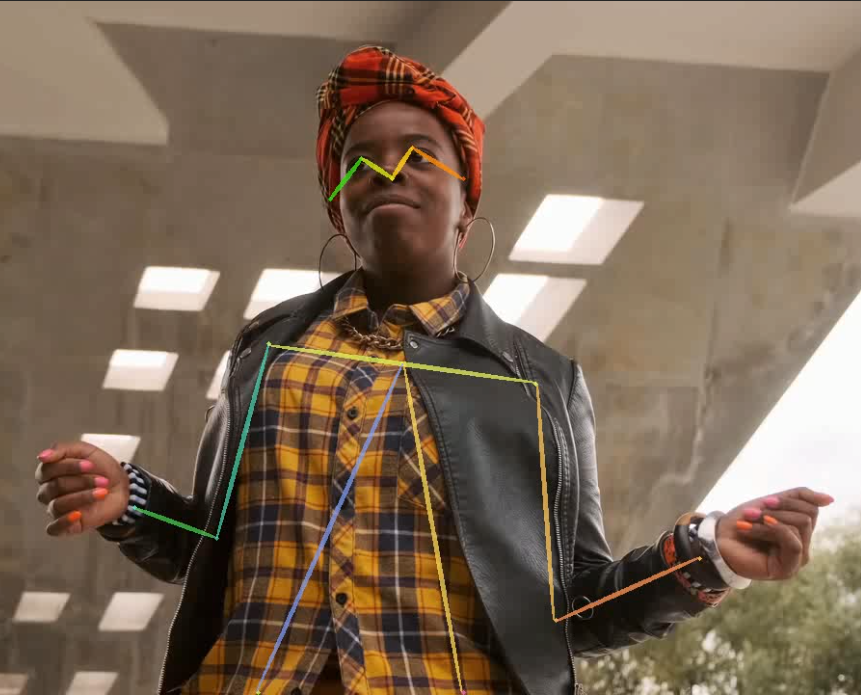
\includegraphics[width=0.45\textwidth]{after_alphapose.png}
			\caption{Результат работы alphapose}
		\end{figure}
	
		\begin{figure}[bhtp]
			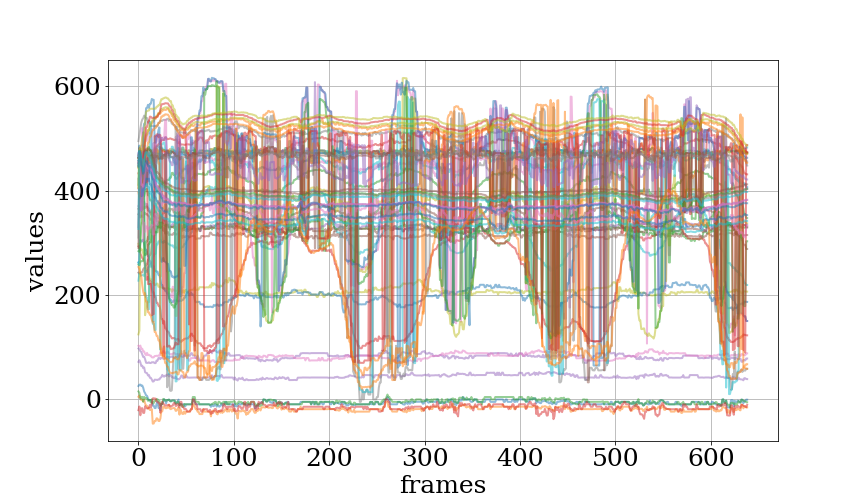
\includegraphics[width=0.55\textwidth]{cyclic_video_data.png}
			\caption{Данные видео-кейпоинтов}
		\end{figure}
		\end{multicols}
		
	\end{frame}

	\begin{frame}{Анализ ошибки}
		\begin{table}[bhtp]
			\fontsize{4pt}{8pt}
			\selectfont
			\centering
			\caption{Сравнение ошибки предсказательной модели в траекторном пространстве и в его подпространстве}
			\label{tbl:space_and_subspace}
			\begin{tabularx}{\textwidth}{c|XXXXXX}
				\hline
				& acc\_z & acc\_y & acc\_x & gyr\_z & gyr\_y & gyr\_x \\
				\hline
				space & 1.053 $\pm$ 2.223 & 0.401 $\pm$ 0.833 & 0.483 $\pm$ 0.825 & 0.084 $\pm$ 0.537 & 0.090 $\pm$ 0.094 & 0.063 $\pm$ 0.295 \\
				subspace & 0.315 $\pm$ 0.461 & 0.043 $\pm$ 0.051 & 0.150 $\pm$ 0.177 & 0.001 $\pm$ 0.001	& 0.015 $\pm$ 0.031 & 0.001 $\pm$ 0.003 \\
				\hline
			\end{tabularx}
		\end{table}

		\begin{table}[bhtp]
			\tiny
			\centering
			\caption{Сравнение различных методов снижения размерности}
			\label{tbl:methods}
			\begin{tabular}{l|c|lll}
				\hline
				\multicolumn{2}{l}{\diaghead{\hskip4cm}{Целевой признак}{Метод}} \vline & PLS-AE & PLS-CCM & PLS \\
				\hline
				\multirow{6}{*}{\rotatebox[origin=c]{90}{cyclic}} & acc\_z & 4.087 & 5.826 & \textbf{4.013} \\
				& acc\_y & \textbf{1.069} & 3.947 & 2.725 \\
				& acc\_x & 4.113 & \textbf{3.257} & 4.358 \\
				& gyr\_z & \textbf{0.949} & 1.074 & 2.067 \\
				& gyr\_y & 3.462 & 4.193 & \textbf{1.401} \\
				& gyr\_x & 1.148 & \textbf{0.511} & 2.671 \\
				\hline
				\multirow{6}{*}{\rotatebox[origin=c]{90}{chaotic}} & acc\_z & 35.675 & 32.448 & \textbf{25.588} \\
				& acc\_y & 15.537 & 15.564 & \textbf{7.540} \\
				& acc\_x & 36.388 & \textbf{32.363} & 38.208 \\
				& gyr\_z & 25.892 & 12.686 & \textbf{6.574} \\
				& gyr\_y & 10.286 & 17.241 & \textbf{3.165} \\
				& gyr\_x & 12.907 & 29.840 & \textbf{3.941} \\
				\hline   
			\end{tabular}
		\end{table}
	\end{frame}

	\begin{frame}{Заключение}
		\begin{enumerate}
			\item Предложен метод согласованного снижения размерности, объединяющий в себе методы PLS и Сугихары
			
			\item Проведён вычислительный эксперимент на данных устройств и видеоряда
			
			\item Получено, что использование данных из видео повышает качество прогнозирования
			
			\item Показано, что прогностическая модель менее устойчива в случае, когда та применяется в траекторном пространстве
		\end{enumerate}
	\end{frame}

\end{document}
